\documentclass[a4paper,10pt]{article}
\usepackage{latexsym}
\usepackage[activeacute,spanish]{babel}
\usepackage{anysize}
\usepackage{float}
\usepackage{graphicx}
\usepackage[utf8]{inputenc}
\usepackage{listings}
\usepackage{mdframed}
\usepackage{color}



\marginsize{2cm}{2cm}{2cm}{2cm}
\author{Felipe V\'asquez 201104535-1 [felipe.vasquezm@alumnos.usm.cl]\\Cecilia Villarroel 201104558-0 [cecilia.villarroel@alumnos.usm.cl]\\ Primer semestre 2014}
\title{ILI 256 - Informe Tarea 3}
\frenchspacing
\begin{document}
\maketitle


\section{Preguntas}



 %Pregunta 1
\subsection{} 
\raggedright Utilizando open visual traceroute se rastrearon las rutas por las que pasan los paquetes que se quieren obtener mediante las direcciones web entregadas.\\ \\

La internet, normalmente, se pensaría que no es de nadie o de todos, por el libre acceso a la información. Sin embargo, su dueño, se podría decir que es el gobierno de Estado Unidos, a través de una organización privada, sin fines de lucro llamada ICANN  (Internet Corporation for Assigned Names and Numbers), la cual administra servidores gigantes en todo el mundo, que permite el traspaso de información entre hosts. Un departamento de ICANN, llamado IANA (Internet Assigned Numbers Authority) es responsable del manejo y coordinación del sistema de nombres de dominio global de la internet (DNS: Domain Name System) y sistema de enumeración para las direcciones IP. \\

\begin{figure}[H]
\centering
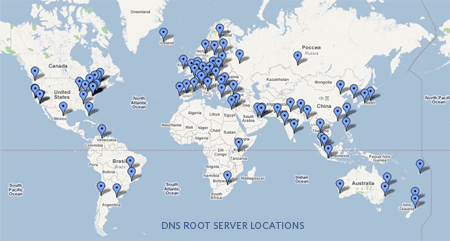
\includegraphics[height=6 cm]{imagenes/root-servers.png}
\caption{Distribución de servidores DNS}
\end{figure} \\ 

La internet, al ser una red de redes, es muy compleja. Está basada en muchos protocolos. La conexión entre un host y el servidor, se hace mediante routers. Estos routers son los que toman las decisiones de que caminos el paquete de información tomara. \\ \\

Los DNS están distribuidos de forma jerarquizada, para evitar el cuello botella y si es que falla, el internet no colapse, entre otros. El cliente pide al DNS una dirección, y lo que hace el DNS es que entrega la dirección IP para poder localizar lo pedido por el usuario. También existe los Local Name servers, los cuales no necesariamente pertenecen a la jerarquía anteriormente mencionada, donde cada proveedor de internet tiene uno, por ejemplo, la universidad, compañía, etc. Si la dirección pedida es desconocida por el servidor local, este envía el paquete de información hacia la jerarquía.\\ \\

Es importante mencionar que la internet, por muy no física que se sienta, esta nos llega a través de cables. Las conexiones intercontinentales, se hacen a través de cables que están sumergidos en los océanos (véase figura 2)\\

\begin{figure}[H]
\centering
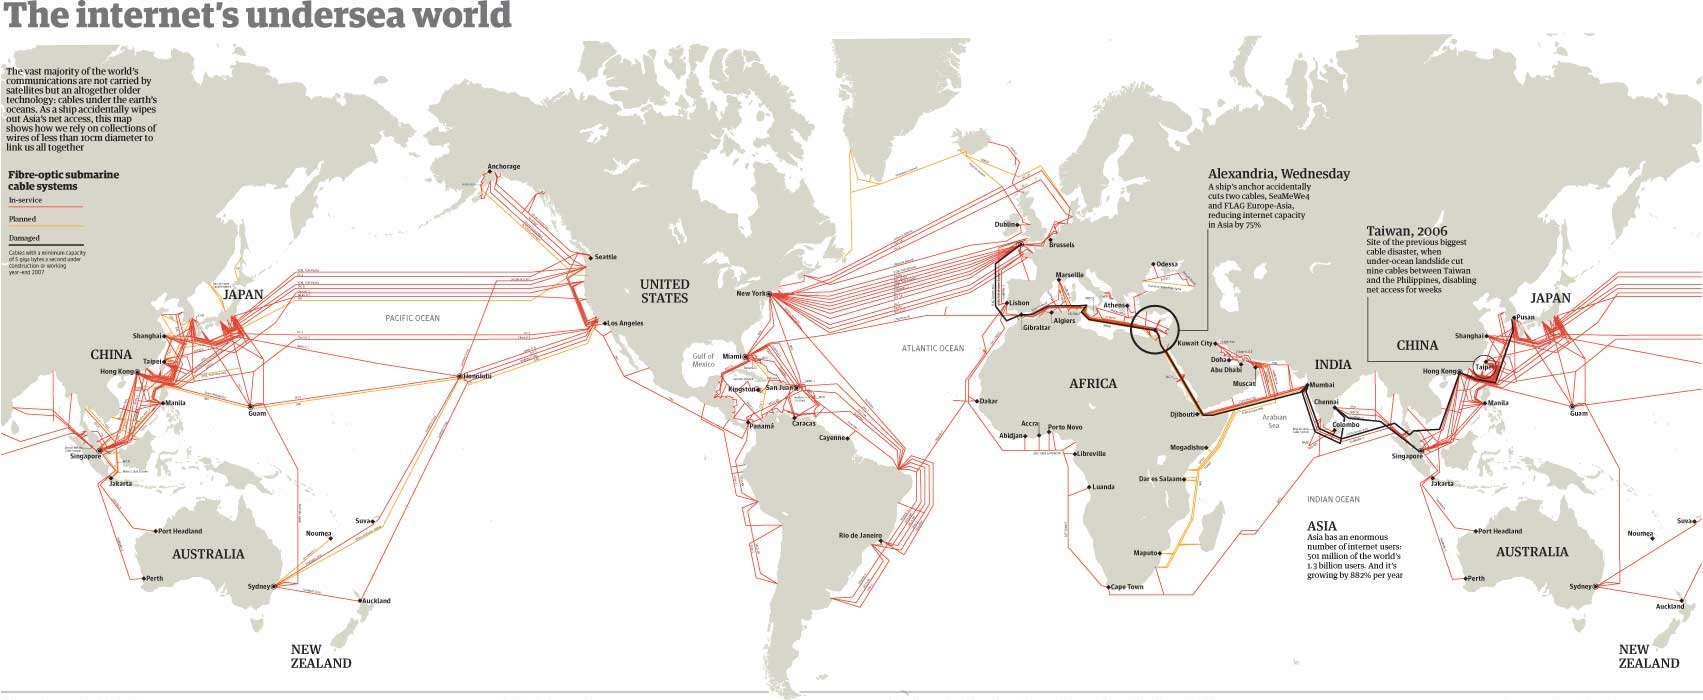
\includegraphics[height=7 cm]{imagenes/seacable.png}
\caption{Cables intercontientales de la Internet}
\end{figure} \\ 

Los enlaces internacionales que tiene Chile, para conectarse a internet, son a través de cables de fibra óptica: \\ \\

\begin{itemize}
  \item Panamericano (PanAm), con conexión en Arica.
  \item South America-1 (Sam-1), con conexión en Arica y Valparaíso.
  \item South American Crossing (SAC) / Latin American Nautilus (LAN), con conexión en Valparaíso.
\end{itemize}


Ademas de estos, la conexión exterior se complementa vía satélite a través de los siguientes telepuertos: \\ \\

\begin{itemize}
  \item (televisión) Curacaví, de TuVes HD.
  \item (televisión) Valdivia, de Telefónica del Sur.
  \item (comunicaciones) Longovilo, de Entel Chile
  \item (comunicaciones) Santiago, de Movistar.
\end{itemize}
\\

A continuación se muestran imágenes de lo sucedido cuando se pide una dirección de enlace (la solicitud de enlaces web fue hecho desde una ISP local (VTR), en Santiago):\\ 
\begin{itemize}
 \item \textbf{\textsl{ http://moodle.inf.cl/}}\\

\begin{figure}[H]
\centering
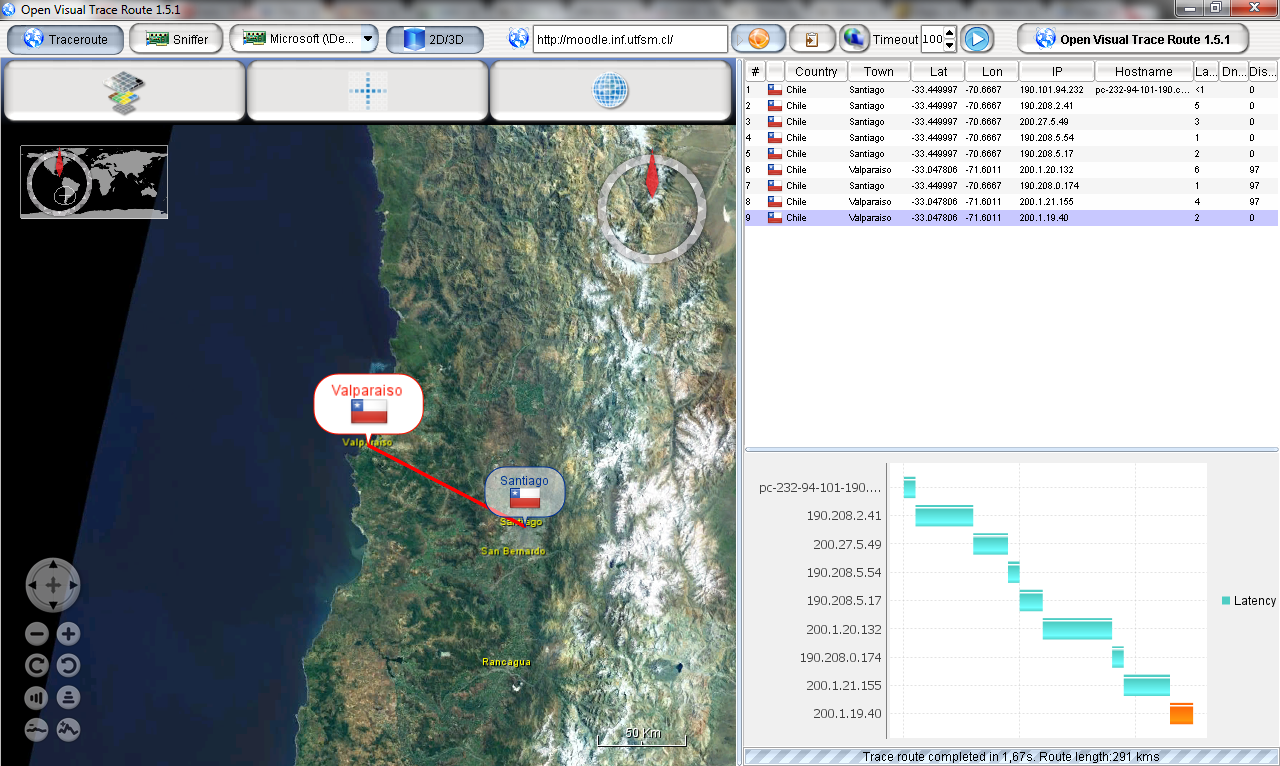
\includegraphics[height=8 cm]{imagenes/enlace1.png}
\caption{Imagen de la ruta que toma conseguir el enlace http://moodle.inf.cl/ }
\end{figure} \\ 

En esta primera imagen del OVT, se puede observar que el paquete no ha salido de Chile, es decir, en Chile existe un DNS local, el cual reconoce la página que se pide, y lo manda ( a través de varios saltos) al servidor local de la universidad (en Valparaíso). \\

 \item  \textbf{\textsl{http://google.cl/}}\\

\begin{figure}[H]
\centering
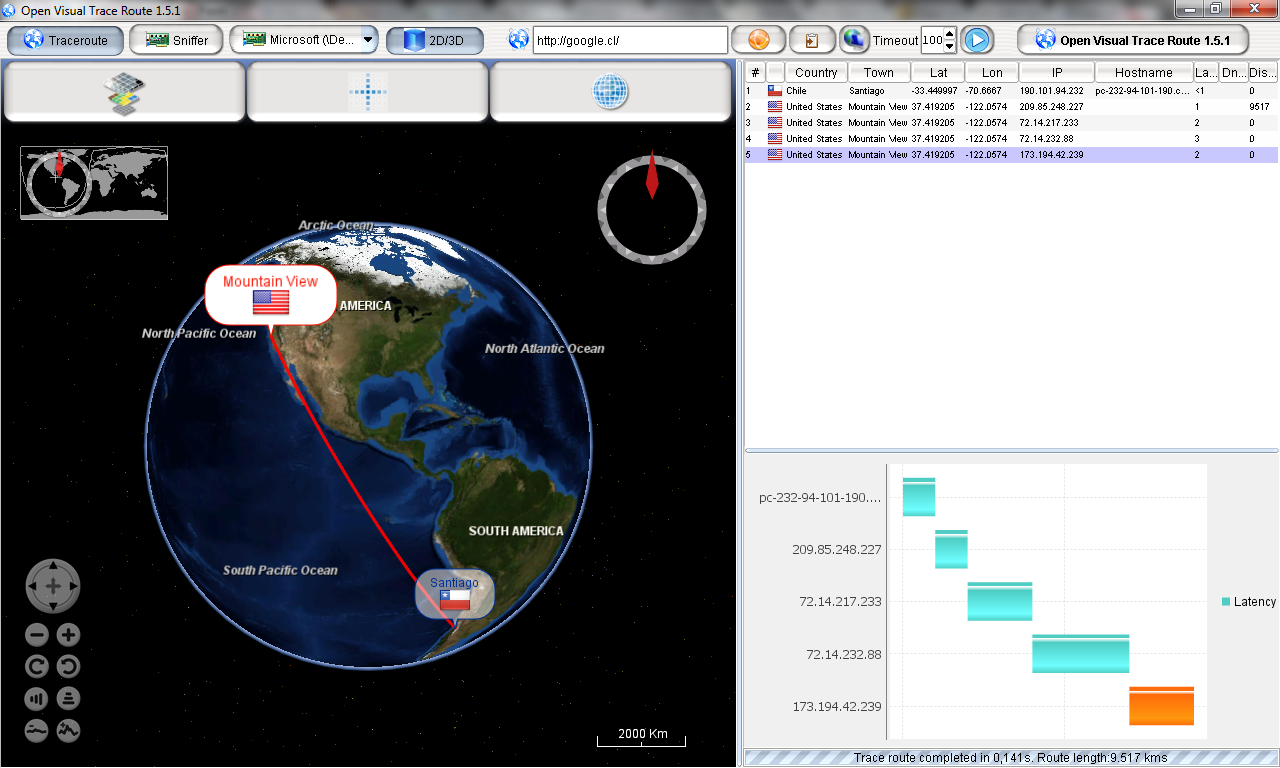
\includegraphics[height=8 cm]{imagenes/enlace2.png}
\caption{Imagen de la ruta que toma conseguir el enlace http://google.cl/ }
\end{figure} \\ 

En esta imagen, se puede observar que el paquete es enviado a Mountain View en Estados Unidos, para luego hacer 4 saltos más, hasta llegar al servidor.\\

 \item  \textbf{\textsl{http://cime.cl/}}\\



\begin{figure}[H]
\centering
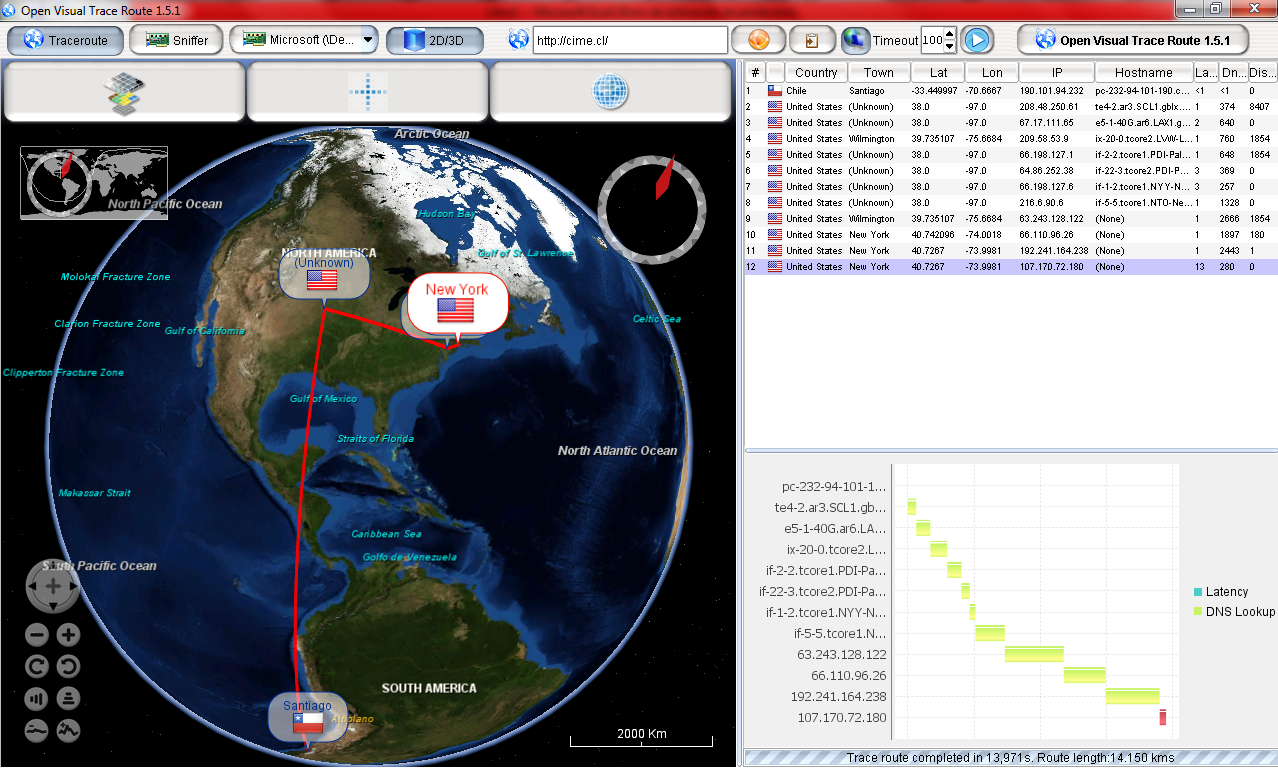
\includegraphics[height=8 cm]{imagenes/enlace3.png}
\caption{Imagen de la ruta que toma conseguir el enlace http://cime.cl/ }
\end{figure} \\ 

En esta imagen, se puede observar que el paquete es enviado desde Chile, para luego pegar varios saltos por Estados Unidos, para finalmente llegar a un servidor en Nueva York, donde se encuentra la pagina solicitada.\\

 \item  \textbf{\textsl{http://wikipedia.com/}}\\



\begin{figure}[H]
\centering
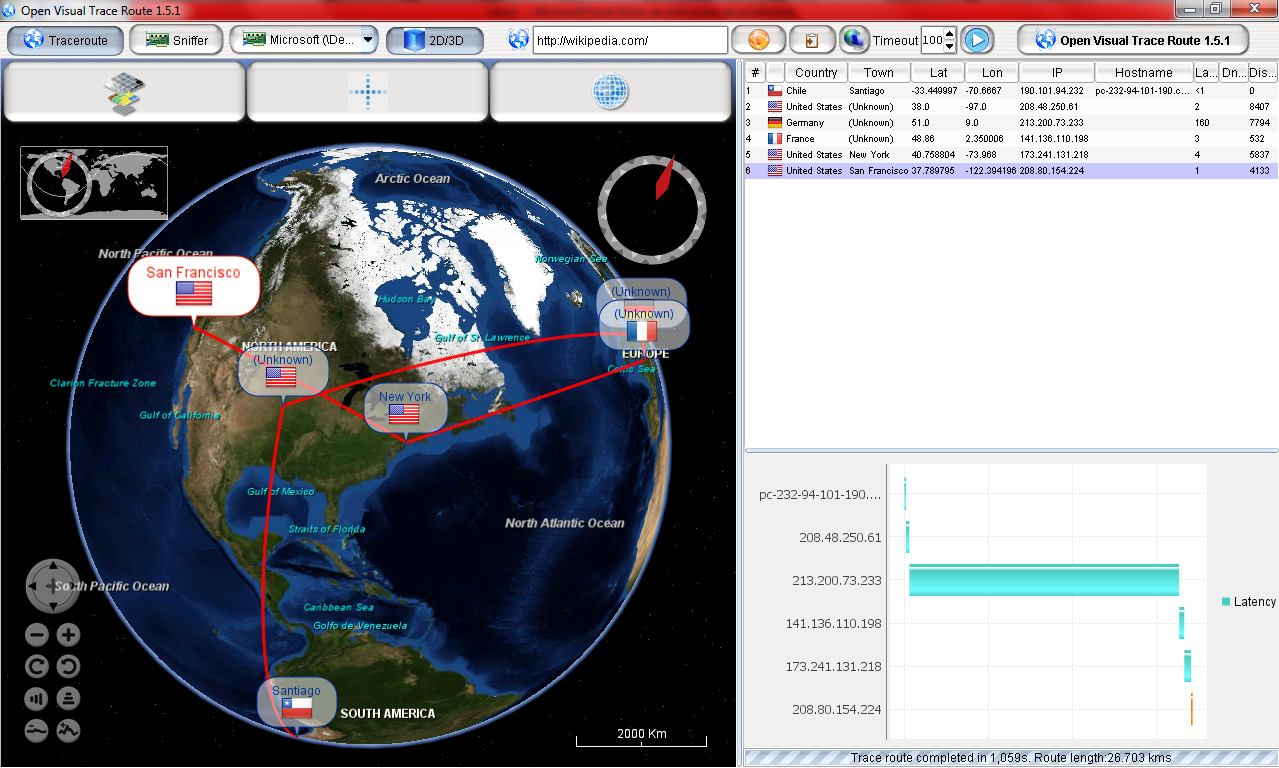
\includegraphics[height=8 cm]{imagenes/enlace4.png}
\caption{Imagen de la ruta que toma conseguir el enlace http://wikipedia.com/ }
\end{figure} \\ 

En esta imagen, se puede observar que el paquete nuevamente es enviado a Estados Unidos (ciudad desconocida) para luego saltar a Alemania, luego a Francia, luego vuelve a los Estados Unidos (Nueva York) y finalmente a San Francisco del mismo país.\\
 \item \textbf{\textsl{http://www.chile.embassy.gov.au/}}\\

\begin{figure}[H]
\centering
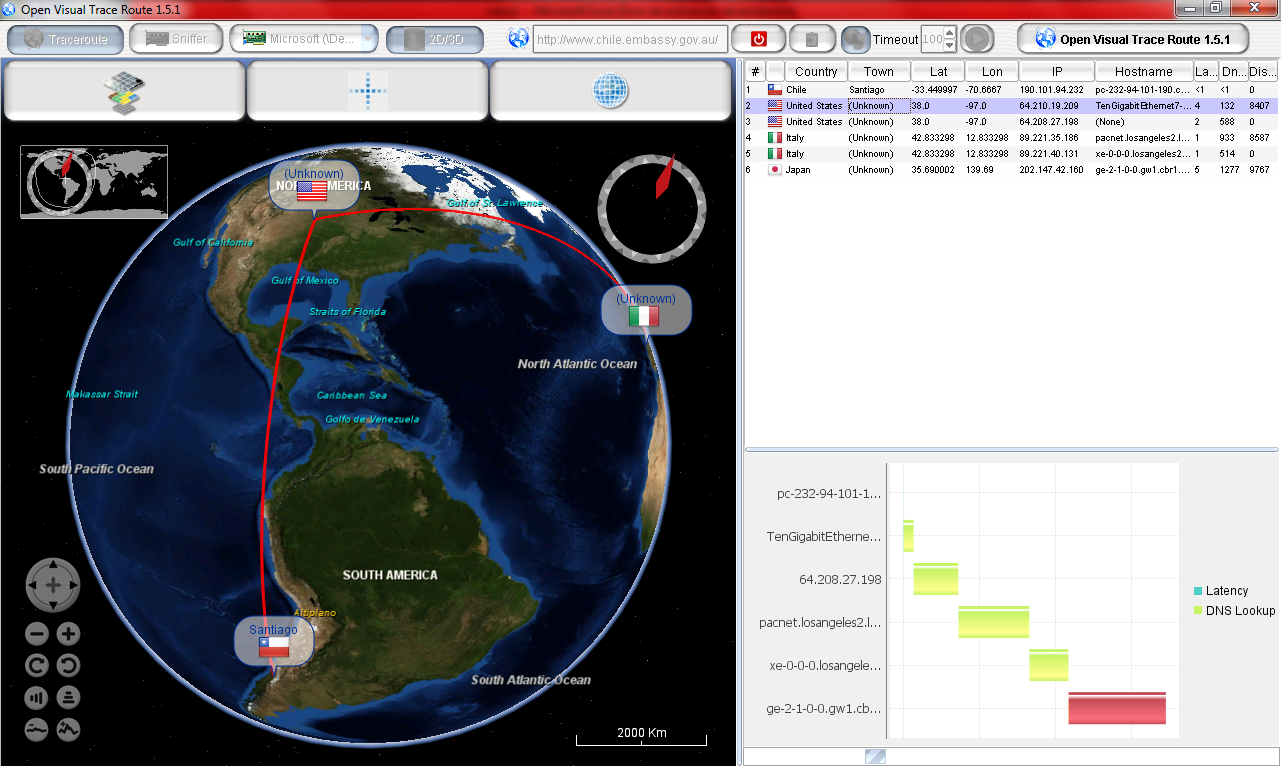
\includegraphics[height=8 cm]{imagenes/enlace51.png}
\caption{Imagen de la ruta que toma conseguir el enlace http://www.chile.embassy.gov.au/ }
\end{figure} \\ 

\begin{figure}[H]
\centering
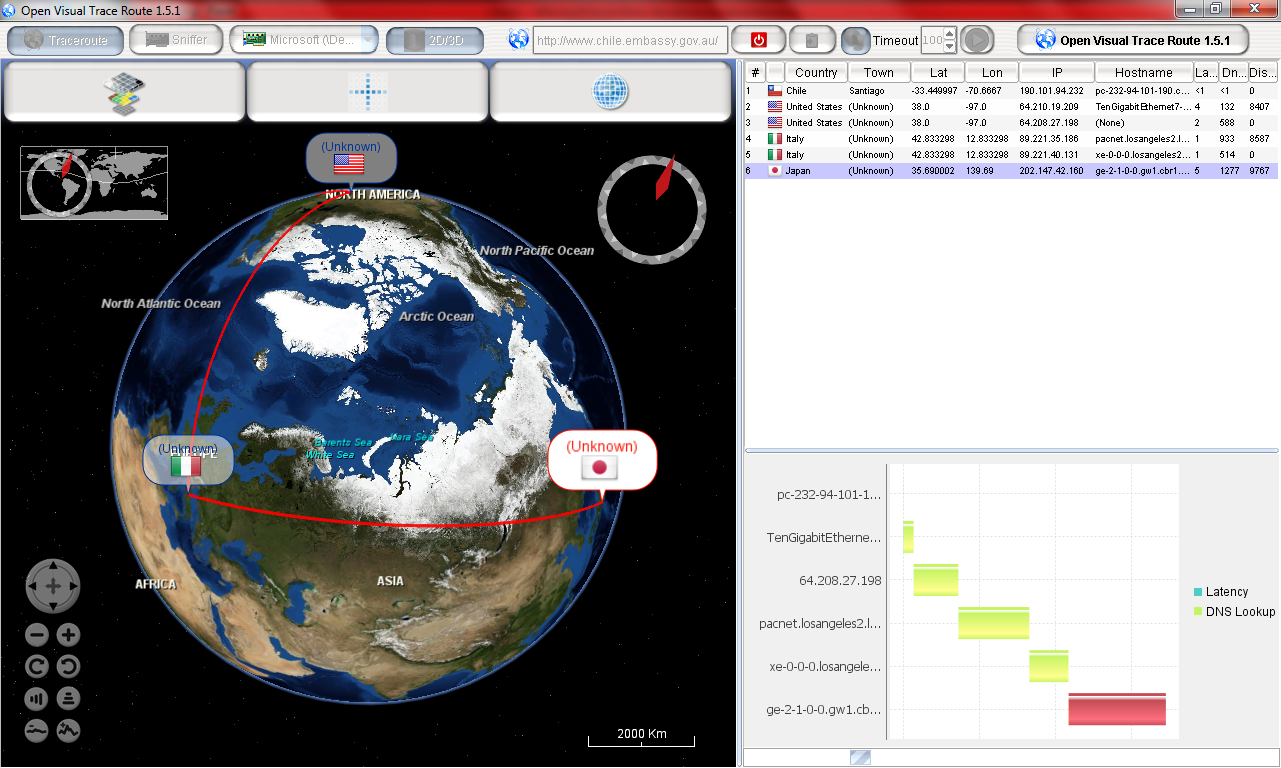
\includegraphics[height=8 cm]{imagenes/enlace52.png}
\caption{Imagen de la ruta que toma conseguir el enlace http://www.chile.embassy.gov.au/ }
\end{figure} \\ \\


En estas imágenes se puede observar los saltos realizados, de Chile a Estados Unidos, luego hace otro salto dentro de Estados unidos, para luego saltar a Italia, donde hace un salto más dentro del mismo país, para terminar en Japón. Vale la pena mencionar que por mucho time out que se diera, este lugar no parecía ser su destino final, lo que probablemente era debido a un firewall en algún servidor en Japón.\\

\end{itemize}


%Pregunta 2
\subsection{}Para cada iteración de algoritmo de ruteo Vector-Distancia se aplica la ecuación de Bellman-Ford, solo se muestra la aplicación de esta ecuación para las iteraciones de la matriz correspondiente al Router A, dado que el procedimiento es el mismo para los demás Router’s de acuerdo a sus valores. Para optimizar el espacio se generan las 9 matrices correspondientes a cada Router y se itera sobre estas mismas utilizando diferentes colores para cada iteración, donde se obtiene lo siguiente:\\

\raggedright \textbf{1\° Iteración:} \\ \\ \\
En la primera iteración, cada router solo conoce la información asociada a sus vecinos directos.\\ \\
 {\color{red}2\° Iteración:}\\ \\

\begin{equation*}\\

D_A (B)=min⁡\{c(A,B)+D_B (B)\}=min⁡\{1+0\}=1\\
D_A (C)=min⁡\{c(A,B)+D_B (C)\}=min⁡\{1+9\}=10\\
D_A (D)=min⁡\{c(A,I)+D_I (D)\}=min⁡\{10+2\}=12\\
D_A (E)=min⁡\{c(A,B)+D_B (E),c(A,I)+D_I (E)\}=min⁡\{1+8,10+1\}=9\\
D_A (G)=min⁡\{c(A,G)+D_G (G)\}=min⁡\{4+0\}=4\\
D_A (H)=min⁡\{c(A,G)+D_G (H),c(A,I)+D_I (H)\}=min⁡\{4+7,10+3\}=11\\
D_A (I)=min\{c(A,I)+D_I (I)\}=min⁡\{10+0\}=10\\



\end{equation*}
\\

{\color{blue}3\° Iteración:}\\ \\

\begin{equation*}\\

D_A (B)=min⁡⁡\{c(A,B)+D_B (B),c(A,G)+D_G (B),c(A,I)+D_I (B)\}\\
D_A (B)=min⁡⁡\{1+0,4+5,10+9\}=1\\
D_A (C)=min⁡⁡\{c(A,B)+D_B (C),c(A,I)+D_I (C)\}=min⁡\{1+9,10+4⁡\}=10\\
D_A (D)=min⁡⁡\{c(A,B)+D_B (D),c(A,I)+D_I (D)\}=min\{1+11,10+2\}=12\\
D_A (E)=min⁡⁡\{c(A,B)+D_B (E),c(A,I)+D_I (E)\}=min⁡\{1+8,10+1\}=9\\
D_A (F)=min⁡⁡\{c(A,B)+D_B (F),c(A,G)+D_G (F),c(A,I)+D_I (F)\}\\
D_A (F)=min⁡⁡\{1+10,4+13,10+3\}=11\\
D_A (G)=min⁡⁡\{c(A,B)+D_B (G),c(A,G)+D_G (G),c(A,I)+D_I (G)\}\\
D_A (G)=min⁡⁡\{1+5,4+0,10+10\}=4\\
D_A (H)=min⁡⁡\{c(A,G)+D_G (H),c(A,I)+D_I (H)\}=min⁡\{4+7,10+3\}=11\\
D_A (I)=min⁡⁡\{c(A,B)+D_B (I),c(A,G)+D_G (I),c(A,I)+D_I (I)\}\\
D_A (I)=min⁡⁡\{1+9,4+10,10+0\}=10\\


\end{equation*}
\\

{\color{green}4\° Iteración:}\\ \\

\begin{equation*}\\

D_A (B)=min\{⁡c(A,B)+D_B (B),c(A,G)+D_G (B),c(A,I)+D_I (B)\}\\
D_A (B)=min⁡\{1+0,4+5,10+9\}=1\\
D_A (C)=min\{c(A,B)+D_B (C),c(A,G)+D_G (C),c(A,I)+D_I (C)\}\\
D_A (C)=min\{1+9,4+14,10+4\}=10\\
D_A (D)=min\{c(A,B)+D_B (D),c(A,G)+D_G (D),c(A,I)+D_I (D)\}\\
D_A (D)=min\{1+11,4+12,10+2\}=12\\
D_A (E)=min⁡\{⁡c(A,B)+D_B (E),c(A,I)+D_I (E)\}\\
D_A (E)=min⁡\{⁡1+8,10+1\}=9\\
D_A (F)=min⁡\{⁡c(A,B)+D_B (F),c(A,G)+D_G (F),c(A,I)+D_I (F)\}\\
D_A (F)=min⁡\{⁡1+10,4+13,10+3\}=11\\
D_A (G)=min\{c(A,B)+D_B (G),c(A,G)+D_G (G),c(A,I)+D_I (G)\}\\
D_A (G)=min⁡\{1+5,4+0,10+10\}=4\\
D_A (H)=min\{c(A,B)+D_B (H),c(A,G)+D_G (H),c(A,I)+D_I (H)\}\\
D_A (H)=min⁡\{1+12,4+7,10+3\}=11\\
D_A (I)=min⁡\{c(A,B)+D_B (I),c(A,G)+D_G (I),c(A,I)+D_I (I)\}\\
D_A (I)=min⁡\{1+9,4+10,10+0\}=10\\



\end{equation*}
\\


\begin{table}[H]
\centering
\begin{tabular}{|c|c|c|c|c|c|c|c|c|c|} \hline
    & A & B & C & D & E & F & G & H & I  \\\hline
A & $ 0,{\color{red}0,}{\color{blue}0,}{\color{green}0} $ & $1,{\color{red}1,}{\color{blue}1,}{\color{green}1} $ & $ \infty,{\color{red}10,}{\color{blue}10,}{\color{green}10} $ & $ \infty,{\color{red}12,}{\color{blue}12,}{\color{green}12} $ & $ \infty,{\color{red}9,}{\color{blue}9,}{\color{green}9} $ & $ \infty,{\color{blue}11,}{\color{green}11} $ & $ 4,{\color{red}4,}{\color{blue}4,}{\color{green}4} $ & $ \infty,{\color{red}11,}{\color{blue}11,}{\color{green}11} $ & $10,{\color{red}10,}{\color{blue}10,}{\color{green}10} $ \\\hline
B & $ \infty,{\color{red}1,}{\color{blue}1,}{\color{green}1} $ & $ \infty,{\color{red}0,}{\color{blue}0,}{\color{green}0} $ & $ \infty,{\color{red}9,}{\color{blue}9,}{\color{green}9} $ & $ \infty,{\color{blue}11,}{\color{green}11} $ & $ \infty,{\color{red}8,}{\color{blue}8,}{\color{green}8} $ & $ \infty,{\color{blue}10,}{\color{green}10} $ & $ \infty,{\color{blue}5,}{\color{green}5} $ & $ \infty,{\color{green}12} $ & $ \infty,{\color{blue}9,}{\color{green}9} $ \\\hline
C & $ \infty $ & $ \infty $ & $ \infty $ & $ \infty $ & $ \infty $ & $ \infty $ & $ \infty $ & $ \infty $ & $ \infty $ \\\hline
D & $ \infty $ & $ \infty $ & $ \infty $ & $ \infty $ & $ \infty $ & $ \infty $ & $ \infty $ & $ \infty $ & $ \infty $ \\\hline
E & $ \infty $ & $ \infty $ & $ \infty $ & $ \infty $ & $ \infty $ & $ \infty $ & $ \infty $ & $ \infty $ & $ \infty $ \\\hline
F & $ \infty $ & $ \infty $ & $ \infty $ & $ \infty $ & $ \infty $ & $ \infty $ & $ \infty $ & $ \infty $ & $ \infty $ \\\hline
G & $ \infty,{\color{red}4,}{\color{blue}4,}{\color{green}4} $ & $ \infty,{\color{blue}5,}{\color{green}5} $ & $ \infty,{\color{green}14} $ & $ \infty,{\color{green}12} $ & $ \infty,{\color{green}11} $ & $ \infty,{\color{blue}13,}{\color{green}13} $ & $ \infty,{\color{red}0,}{\color{blue}0,}{\color{green}0} $ & $ \infty,{\color{red}7,}{\color{blue}7,}{\color{green}7} $ & $ \infty,{\color{blue}10,}{\color{green}10} $ \\\hline
H & $ \infty $ & $ \infty $ & $ \infty $ & $ \infty $ & $ \infty $ & $ \infty $ & $ \infty $ & $ \infty $ & $ \infty $ \\\hline
I & $  \infty,{\color{red}10,}{\color{blue}10,}{\color{green}10}$ & $ \infty,{\color{blue}9,}{\color{green}9} $ & $ \infty,{\color{blue}4,}{\color{green}4} $ & $ \infty,{\color{red}2,}{\color{blue}2,}{\color{green}2} $ & $ \infty,{\color{red}1,}{\color{blue}1,}{\color{green}1} $ & $ \infty,{\color{blue}3,}{\color{green}3} $ & $ \infty,{\color{blue}10,}{\color{green}10} $ & $ \infty,{\color{red}3,}{\color{blue}3,}{\color{green}3} $ & $  \infty,{\color{red}0,}{\color{blue}0,}{\color{green}0}$ \\\hline
\end{tabular}
\caption{Router A}
\end{table} \\



\begin{table}[H]
\centering
\begin{tabular}{|c|c|c|c|c|c|c|c|c|c|} \hline
 & A & B & C & D & E & F & G & H & I  \\\hline
A & $ \infty,{\color{red}0,}{\color{blue}0,}{\color{green}0} $ & $\infty,{\color{red}1,}{\color{blue}1,}{\color{green}1} $ & $\infty,{\color{blue}10,}{\color{green}10} $ & $\infty,{\color{blue}12,}{\color{green}12} $ & $\infty,{\color{blue}9,}{\color{green}9} $ & $\infty,{\color{green}11} $ & $\infty,{\color{red}4,}{\color{blue}4,}{\color{green}4} $ & $\infty,{\color{blue}11,}{\color{green}11} $ & $\infty,{\color{red}10,}{\color{blue}10,}{\color{green}10} $ \\\hline
B & $1,{\color{red}1,}{\color{blue}1,}{\color{green}1} $ & $0,{\color{red}0,}{\color{blue}0,}{\color{green}0} $ & $9,{\color{red}9,}{\color{blue}9,}{\color{green}9} $ & $\infty,{\color{red}11,}{\color{blue}11,}{\color{green}11}$ & $8,{\color{red}8,}{\color{blue}8,}{\color{green}8} $ & $\infty,{\color{red}10,}{\color{blue}10,}{\color{green}10} $ & $\infty,{\color{red}5,}{\color{blue}5,}{\color{green}5} $ & $\infty,{\color{blue}12,}{\color{green}12} $ & $\infty,{\color{red}9,}{\color{blue}9,}{\color{green}9} $ \\\hline
C & $\infty,{\color{blue}10,}{\color{green}10} $ & $\infty,{\color{red}9,}{\color{blue}9,}{\color{green}9} $ & $\infty,{\color{red}0,}{\color{blue}0,}{\color{green}0} $ & $\infty,{\color{red}2,}{\color{blue}2,}{\color{green}2} $ & $\infty,{\color{blue}11,}{\color{green}5} $ & $\infty,{\color{blue}6,}{\color{green}6} $ & $\infty,{\color{green}14} $ & $\infty,{\color{green}7} $ & $\infty,{\color{blue}4,}{\color{green}4} $ \\\hline
D & $\infty $ & $\infty $ & $\infty $ & $\infty $ & $\infty $ & $\infty $ & $\infty $ & $\infty $ & $\infty $ \\\hline
E & $\infty,{\color{blue}9,}{\color{green}9} $ & $\infty,{\color{red}8,}{\color{blue}8,}{\color{green}8} $ & $\infty,{\color{blue}11,}{\color{green}5} $ & $\infty,{\color{red}9,}{\color{blue}3,}{\color{green}3} $ & $\infty,{\color{red}0,}{\color{blue}0,}{\color{green}0} $ & $\infty,{\color{red}2,}{\color{blue}2,}{\color{green}2} $ & $\infty,{\color{green}11} $ & $\infty,{\color{green}4} $ & $\infty,{\color{red}1,}{\color{blue}1,}{\color{green}1} $ \\\hline
F & $\infty $ & $\infty $ & $\infty $ & $\infty $ & $\infty $ & $\infty $ & $\infty $ & $\infty $ & $\infty $ \\\hline
G & $\infty $ & $\infty $ & $\infty $ & $\infty $ & $\infty $ & $\infty $ & $\infty $ & $\infty $ & $\infty $ \\\hline
H & $\infty $ & $\infty $ & $\infty $ & $\infty $ & $\infty $ & $\infty $ & $\infty $ & $\infty $ & $\infty $ \\\hline
I & $\infty $ & $\infty $ & $\infty $ & $\infty $ & $\infty $ & $\infty $ & $\infty $ & $\infty $ & $\infty $ \\\hline
\end{tabular}
\caption{Router B}
\end{table} \\



\begin{table}[H]
\centering
\begin{tabular}{|c|c|c|c|c|c|c|c|c|c|} \hline
 & A & B & C & D & E & F & G & H & I  \\\hline
A & $ \infty $ & $\infty $ & $\infty $ & $\infty $ & $\infty $ & $\infty $ & $\infty $ & $ \infty$ & $\infty $ \\\hline
B & $\infty,{\color{red}1,}{\color{blue}1,}{\color{green}1}$ & $\infty,{\color{red}0,}{\color{blue}0,}{\color{green}0} $ & $\infty,{\color{red}9,}{\color{blue}9,}{\color{green}9} $ & $ \infty,{\color{blue}11,}{\color{green}11}$ & $\infty,{\color{red}8,}{\color{blue}8,}{\color{green}8} $ & $ \infty,{\color{blue}10,}{\color{green}10}$ & $\infty,{\color{blue}5,}{\color{green}5} $ & $ \infty,{\color{green}12}$ & $\infty,{\color{blue}9,}{\color{green}9} $  \\\hline
C & $ \infty,{\color{red}10,}{\color{blue}10,}{\color{green}10}$ & $9,{\color{red}9,}{\color{blue}9,}{\color{green}9} $ & $0,{\color{red}0,}{\color{blue}0,}{\color{green}0} $ & $2,{\color{red}2,}{\color{blue}2,}{\color{green}2} $ & $ \infty,{\color{red}11,}{\color{blue}5,}{\color{green}5}$ & $\infty,{\color{red}6,}{\color{blue}6,}{\color{green}6} $ & $\infty,{\color{blue}14,}{\color{green}14} $ & $\infty,{\color{blue}7,}{\color{green}7} $ & $ \infty,{\color{red}4,}{\color{blue}4,}{\color{green}4}$ \\\hline
D & $ \infty,{\color{green}12}$ & $\infty,{\color{blue}11,}{\color{green}11} $ & $\infty,{\color{red}2,}{\color{blue}2,}{\color{green}2} $ & $\infty,{\color{red}0,}{\color{blue}0,}{\color{green}0} $ & $\infty,{\color{red}9,}{\color{blue}3,}{\color{green}3} $ & $\infty,{\color{red}4,}{\color{blue}4,}{\color{green}4} $ & $ \infty,{\color{green}12}$ & $\infty,{\color{blue}5,}{\color{green}5} $ & $\infty,{\color{red}2,}{\color{blue}2,}{\color{green}2} $ \\\hline
E & $ \infty$ & $\infty $ & $\infty $ & $\infty $ & $\infty $ & $\infty $ & $ \infty$ & $\infty $ & $\infty $ \\\hline
F & $ \infty$ & $\infty $ & $\infty $ & $\infty $ & $\infty $ & $\infty $ & $ \infty$ & $\infty $ & $\infty $ \\\hline
G & $ \infty$ & $\infty $ & $\infty $ & $\infty $ & $\infty $ & $\infty $ & $ \infty$ & $\infty $ & $\infty $ \\\hline
H & $ \infty$ & $\infty $ & $\infty $ & $\infty $ & $\infty $ & $\infty $ & $ \infty$ & $\infty $ & $\infty $ \\\hline
I & $ \infty$ & $\infty $ & $ \infty$ & $\infty $ & $ \infty$ & $\infty $ & $ \infty$ & $ \infty$ & $ \infty$ \\\hline
\end{tabular}
\caption{Router C}
\end{table} \\

 

\begin{table}[H]
\centering
\begin{tabular}{|c|c|c|c|c|c|c|c|c|c|} \hline
 & A & B & C & D & E & F & G & H & I  \\\hline
A & $ \infty $ & $\infty $ & $ \infty$ & $\infty $ & $\infty $ & $\infty $ & $\infty $ & $\infty $ & $ \infty$ \\\hline
B & $\infty $ & $\infty $ & $ \infty$ & $\infty $ & $ \infty$ & $\infty $ & $ \infty$ & $ \infty$ & $ \infty$ \\\hline
C & $\infty,{\color{blue}10,}{\color{green}10} $ & $\infty,{\color{red}9,}{\color{blue}9,}{\color{green}9} $ & $ \infty,{\color{red}0,}{\color{blue}0,}{\color{green}0}$ & $\infty,{\color{red}2,}{\color{blue}2,}{\color{green}2} $ & $ \infty,{\color{blue}11,}{\color{green}5}$ & $\infty,{\color{blue}6,}{\color{green}6} $ & $ \infty,{\color{green}14}$ & $ \infty,{\color{green}7}$ & $\infty,{\color{blue}4,}{\color{green}4} $ \\\hline
D & $\infty,{\color{blue}12,}{\color{green}12} $ & $\infty,{\color{red}11,}{\color{blue}11,}{\color{green}11} $ & $ 2,{\color{red}2,}{\color{blue}2,}{\color{green}2}$ & $0,{\color{red}0,}{\color{blue}0,}{\color{green}0} $ & $9,{\color{red}3,}{\color{blue}3,}{\color{green}3} $ & $ 4,{\color{red}4,}{\color{blue}4,}{\color{green}4}$ & $\infty,{\color{blue}12,}{\color{green}12} $ & $\infty,{\color{red}5,}{\color{blue}5,}{\color{green}5} $ & $2,{\color{red}2,}{\color{blue}2,}{\color{green}2} $ \\\hline
E & $\infty,{\color{blue}9,}{\color{green}9} $ & $\infty,{\color{red}8,}{\color{blue}8,}{\color{green}8} $ & $ \infty,{\color{blue}11,}{\color{green}5}$ & $\infty,{\color{red}9,}{\color{blue}3,}{\color{green}3} $ & $\infty,{\color{red}0,}{\color{blue}0,}{\color{green}0} $ & $\infty,{\color{red}2,}{\color{blue}2,}{\color{green}2} $ & $ \infty,{\color{green}11}$ & $ \infty,{\color{green}4}$ & $\infty,{\color{red}1,}{\color{blue}1,}{\color{green}1} $ \\\hline
F & $\infty,{\color{green}11} $ & $\infty,{\color{blue}10,}{\color{green}10} $ & $ \infty,{\color{blue}6,}{\color{green}6}$ & $\infty,{\color{red}4,}{\color{blue}4,}{\color{green}4} $ & $\infty,{\color{red}2,}{\color{blue}2,}{\color{green}2} $ & $\infty,{\color{red}0,}{\color{blue}0,}{\color{green}0} $ & $ \infty,{\color{blue}13,}{\color{green}13}$ & $ \infty,{\color{red}6,}{\color{blue}6,}{\color{green}6}$ & $\infty,{\color{blue}3,}{\color{green}3} $ \\\hline
G & $\infty $ & $\infty $ & $ \infty$ & $\infty $ & $\infty $ & $\infty $ & $ \infty$ & $ \infty$ & $\infty $ \\\hline
H & $\infty $ & $\infty $ & $ \infty$ & $\infty $ & $\infty $ & $\infty $ & $ \infty$ & $ \infty$ & $\infty $ \\\hline
I & $ \infty,{\color{red}10,}{\color{blue}10,}{\color{green}10}$ & $\infty,{\color{blue}9,}{\color{green}9} $ & $ \infty,{\color{blue}4,}{\color{green}4}$ & $\infty,{\color{red}2,}{\color{blue}2,}{\color{green}2} $ & $ \infty,{\color{red}1,}{\color{blue}1,}{\color{green}1}$ & $ \infty,{\color{blue}3,}{\color{green}3}$ & $ \infty,{\color{blue}10,}{\color{green}10}$ & $\infty,{\color{red}3,}{\color{blue}3,}{\color{green}3} $ & $ \infty,{\color{red}0,}{\color{blue}0,}{\color{green}0}$ \\\hline
\end{tabular}
\caption{Router D}
\end{table} \\



\begin{table}[H]
\centering
\begin{tabular}{|c|c|c|c|c|c|c|c|c|c|} \hline
 & A & B & C & D & E & F & G & H & I  \\\hline
A & $ \infty $ & $ \infty$ & $ \infty$ & $ \infty$ & $ \infty$ & $\infty $ & $\infty$ & $\infty $ & $ \infty$ \\\hline
B & $\infty,{\color{red}1,}{\color{blue}1,}{\color{green}1} $ & $ \infty,{\color{red}0,}{\color{blue}0,}{\color{green}0}$ & $ \infty,{\color{red}9,}{\color{blue}9,}{\color{green}9}$ & $ \infty,{\color{blue}11,}{\color{green}11}$ & $ \infty,{\color{red}8,}{\color{blue}8,}{\color{green}8}$ & $\infty,{\color{blue}10,}{\color{green}10} $ & $\infty,{\color{blue}5,}{\color{green}5}$ & $\infty,{\color{green}12} $ & $ \infty,{\color{blue}9,}{\color{green}9}$ \\\hline
C & $\infty $ & $ \infty$ & $ \infty$ & $ \infty$ & $ \infty$ & $\infty $ & $\infty $ & $\infty $ & $ \infty$ \\\hline
D & $\infty,{\color{green}12}$ & $ \infty,{\color{blue}11,}{\color{green}11}$ & $ \infty,{\color{red}2,}{\color{blue}2,}{\color{green}2}$ & $ \infty,{\color{red}0,}{\color{blue}0,}{\color{green}0}$ & $ \infty,{\color{red}9,}{\color{blue}3,}{\color{green}3}$ & $\infty,{\color{red}4,}{\color{blue}4,}{\color{green}4} $ & $\infty,{\color{green}12} $ & $\infty,{\color{blue}5,}{\color{green}5} $ & $ \infty,{\color{red}2,}{\color{blue}2,}{\color{green}2}$ \\\hline
E & $\infty,{\color{red}9,}{\color{blue}9,}{\color{green}9} $ & $8,{\color{red}8,}{\color{blue}8,}{\color{green}8} $ & $\infty,{\color{red}11,}{\color{blue}5,}{\color{green}5} $ & $9,{\color{red}3,}{\color{blue}3,}{\color{green}3} $ & $ 0,{\color{red}0,}{\color{blue}0,}{\color{green}0}$ & $2,{\color{red}2,}{\color{blue}2,}{\color{green}2} $ & $\infty,{\color{blue}11,}{\color{green}11} $ & $\infty,{\color{red}4,}{\color{blue}4,}{\color{green}4} $ & $1,{\color{red}1,}{\color{blue}1,}{\color{green}1} $ \\\hline
F & $\infty,{\color{green}11} $ & $\infty,{\color{blue}10,}{\color{green}10} $ & $\infty,{\color{blue}6,}{\color{green}6} $ & $ \infty,{\color{red}4,}{\color{blue}4,}{\color{green}4}$ & $ \infty,{\color{red}2,}{\color{blue}2,}{\color{green}2}$ & $\infty,{\color{red}0,}{\color{blue}0,}{\color{green}0} $ & $\infty,{\color{blue}13,}{\color{green}13} $ & $\infty,{\color{red}6,}{\color{blue}6,}{\color{green}6} $ & $ \infty,{\color{blue}3,}{\color{green}3}$ \\\hline
G & $\infty$ & $\infty $ & $\infty $ & $ \infty$ & $ \infty$ & $\infty $ & $\infty $ & $\infty $ & $ \infty$ \\\hline
H & $\infty$ & $\infty$ & $\infty $ & $ \infty$ & $ \infty$ & $\infty $ & $\infty $ & $\infty$ & $ \infty$ \\\hline
I & $ \infty,{\color{red}10,}{\color{blue}10,}{\color{green}10}$ & $\infty,{\color{blue}9,}{\color{green}9} $ & $\infty,{\color{blue}4,}{\color{green}4} $ & $ \infty,{\color{red}2,}{\color{blue}2,}{\color{green}2}$ & $ \infty,{\color{red}1,}{\color{blue}1,}{\color{green}1}$ & $\infty,{\color{blue}3,}{\color{green}3} $ & $ \infty,{\color{blue}10,}{\color{green}10}$ & $ \infty,{\color{red}3,}{\color{blue}3,}{\color{green}3}$ & $ \infty,{\color{red}0,}{\color{blue}0,}{\color{green}0}$ \\\hline
\end{tabular}
\caption{Router E}
\end{table} \\


\begin{table}[H]
\centering
\begin{tabular}{|c|c|c|c|c|c|c|c|c|c|} \hline
 & A & B & C & D & E & F & G & H & I  \\\hline
A & $\infty $ & $\infty $ & $\infty $ & $\infty$ & $\infty$ & $\infty $ & $ \infty$ & $\infty $ & $ \infty$ \\\hline
B & $\infty $ & $\infty $ & $\infty$ & $ \infty$ & $ \infty$ & $\infty $ & $ \infty$ & $\infty $ & $ \infty$ \\\hline
C & $\infty $ & $\infty $ & $\infty$ & $ \infty$ & $ \infty$ & $\infty $ & $ \infty$ & $\infty $ & $ \infty$ \\\hline
D & $\infty,{\color{green}12} $ & $\infty,{\color{blue}11,}{\color{green}11} $ & $\infty,{\color{red}2,}{\color{blue}2,}{\color{green}2}$ & $ \infty,{\color{red}0,}{\color{blue}0,}{\color{green}0}$ & $ \infty,{\color{red}9,}{\color{blue}3,}{\color{green}3}$ & $\infty,{\color{red}4,}{\color{blue}4,}{\color{green}4} $ & $ \infty,{\color{green}12}$ & $\infty,{\color{blue}5,}{\color{green}5} $ & $ \infty,{\color{red}2,}{\color{blue}2,}{\color{green}2}$ \\\hline
E & $\infty,{\color{blue}9,}{\color{green}9} $ & $\infty,{\color{red}8,}{\color{blue}8,}{\color{green}8}$ & $\infty,{\color{blue}11,}{\color{green}5}$ & $ \infty,{\color{red}9,}{\color{blue}3,}{\color{green}3}$ & $ \infty,{\color{red}0,}{\color{blue}0,}{\color{green}0}$ & $\infty,{\color{red}2,}{\color{blue}2,}{\color{green}2} $ & $ \infty,{\color{green}11}$ & $\infty,{\color{green}4} $ & $ \infty,{\color{red}1,}{\color{blue}1,}{\color{green}1}$ \\\hline
F & $\infty,{\color{blue}11,}{\color{green}11} $ & $\infty,{\color{red}10,}{\color{blue}10,}{\color{green}10} $ & $\infty,{\color{red}6,}{\color{blue}6,}{\color{green}6}$ & $4,{\color{red}4,}{\color{blue}4,}{\color{green}4} $ & $2,{\color{red}2,}{\color{blue}2,}{\color{green}2} $ & $0,{\color{red}0,}{\color{blue}0,}{\color{green}0} $ & $\infty,{\color{red}13,}{\color{blue}13,}{\color{green}13} $ & $6,{\color{red}6,}{\color{blue}6,}{\color{green}6} $ & $\infty,{\color{red}3,}{\color{blue}3,}{\color{green}3} $ \\\hline
G & $\infty $ & $\infty $ & $\infty$ & $\infty $ & $ \infty$ & $\infty $ & $ \infty$ & $\infty$ & $ \infty$ \\\hline
H & $\infty,{\color{blue}11,}{\color{green}11} $ & $\infty,{\color{green}12} $ & $\infty,{\color{green}7}$ & $\infty,{\color{blue}5,}{\color{green}5} $ & $ \infty,{\color{blue}4,}{\color{green}4}$ & $\infty,{\color{red}6,}{\color{blue}6,}{\color{green}6} $ & $ \infty,{\color{red}7,}{\color{blue}7,}{\color{green}7}$ & $\infty,{\color{red}0,}{\color{blue}0,}{\color{green}0}$ & $ \infty,{\color{red}3,}{\color{blue}3,}{\color{green}3}$ \\\hline
I & $ \infty$ & $\infty $ & $ \infty$ & $\infty $ & $ \infty$ & $ \infty$ & $ \infty$ & $ \infty$ & $ \infty$ \\\hline
\end{tabular}
\caption{Router F}
\end{table} \\


\begin{table}[H]
\centering
\begin{tabular}{|c|c|c|c|c|c|c|c|c|c|} \hline
 & A & B & C & D & E & F & G & H & I  \\\hline
A & $ \infty,{\color{red}0,}{\color{blue}0,}{\color{green}0} $ & $\infty,{\color{red}1,}{\color{blue}1,}{\color{green}1} $ & $\infty,{\color{blue}10,}{\color{green}10} $ & $\infty,{\color{blue}12,}{\color{green}12} $ & $ \infty,{\color{blue}9,}{\color{green}9}$ & $\infty,{\color{green}11}$ & $ \infty,{\color{red}4,}{\color{blue}4,}{\color{green}4}$ & $\infty,{\color{blue}11,}{\color{green}11} $ & $ \infty,{\color{red}10,}{\color{blue}10,}{\color{green}10}$ \\\hline
B & $\infty $ & $\infty $ & $\infty $ & $\infty $ & $ \infty$ & $\infty$ & $ \infty$ & $\infty $ & $ \infty$ \\\hline
C & $\infty $ & $\infty $ & $\infty $ & $\infty $ & $ \infty$ & $\infty$ & $ \infty$ & $\infty $ & $ \infty$ \\\hline
D & $\infty $ & $\infty $ & $\infty $ & $\infty $ & $ \infty,$ & $\infty $ & $ \infty$ & $\infty $ & $ \infty$ \\\hline
E & $\infty $ & $\infty $ & $\infty $ & $\infty $ & $ \infty$ & $\infty $ & $ \infty$ & $\infty $ & $ \infty$ \\\hline
F & $\infty $ & $\infty $ & $\infty $ & $\infty $ & $ \infty$ & $\infty $ & $ \infty$ & $\infty $ & $ \infty$ \\\hline
G & $4,{\color{red}4,}{\color{blue}4,}{\color{green}4} $ & $\infty,{\color{red}5,}{\color{blue}5,}{\color{green}5} $ & $\infty,{\color{blue}14,}{\color{green}14} $ & $\infty,{\color{blue}12,}{\color{green}12} $ & $\infty,{\color{blue}11,}{\color{green}11} $ & $\infty,{\color{red}13,}{\color{blue}13,}{\color{green}13} $ & $0,{\color{red}0,}{\color{blue}0,}{\color{green}0} $ & $7,{\color{red}7,}{\color{blue}7,}{\color{green}7} $ & $\infty,{\color{red}10,}{\color{blue}10,}{\color{green}10}$ \\\hline
H & $ \infty,{\color{blue}11,}{\color{green}11}$ & $\infty,{\color{green}12} $ & $\infty,{\color{green}7} $ & $\infty,{\color{blue}5,}{\color{green}5} $ & $ \infty,{\color{blue}4,}{\color{green}4}$ & $\infty,{\color{red}6,}{\color{blue}6,}{\color{green}6} $ & $ \infty,{\color{red}7,}{\color{blue}7,}{\color{green}7}$ & $\infty,{\color{red}0,}{\color{blue}0,}{\color{green}0} $ & $ \infty,{\color{red}3,}{\color{blue}3,}{\color{green}3}$ \\\hline
I & $ \infty$ & $\infty $ & $ \infty$ & $ \infty$ & $ \infty$ & $ \infty$ & $ \infty$ & $ \infty$ & $ \infty$ \\\hline
\end{tabular}
\caption{Router G}
\end{table} \\

\begin{table}[H]
\centering
\begin{tabular}{|c|c|c|c|c|c|c|c|c|c|} \hline
 & A & B & C & D & E & F & G & H & I  \\\hline
A & $ \infty $ & $\infty $ & $ \infty$ & $\infty $ & $ \infty$ & $\infty,$ & $ \infty$ & $ \infty$ & $ \infty$ \\\hline
B & $ \infty$ & $\infty $ & $ \infty$ & $\infty $ & $ \infty$ & $\infty $ & $ \infty$ & $ \infty$ & $ \infty$ \\\hline
C & $ \infty$ & $\infty $ & $ \infty$ & $\infty $ & $ \infty$ & $\infty $ & $ \infty$ & $ \infty$ & $ \infty$ \\\hline
D & $ \infty$ & $\infty $ & $ \infty$ & $\infty $ & $ \infty$ & $\infty $ & $ \infty$ & $ \infty$ & $ \infty$ \\\hline
E & $ \infty$ & $\infty $ & $ \infty$ & $\infty $ & $ \infty$ & $\infty $ & $ \infty$ & $ \infty$ & $ \infty$ \\\hline
F & $ \infty,{\color{green}11}$ & $\infty,{\color{blue}10,}{\color{green}10} $ & $ \infty,{\color{blue}6,}{\color{green}6}$ & $\infty,{\color{red}4,}{\color{blue}4,}{\color{green}4} $ & $ \infty,{\color{red}2,}{\color{blue}2,}{\color{green}2}$ & $\infty,{\color{red}0,}{\color{blue}0,}{\color{green}0} $ & $ \infty,{\color{blue}13,}{\color{green}13}$ & $ \infty,{\color{red}6,}{\color{blue}6,}{\color{green}6}$ & $ \infty,{\color{blue}3,}{\color{green}3}$ \\\hline
G & $ \infty,{\color{red}4,}{\color{blue}4,}{\color{green}4}$ & $\infty,{\color{blue}5,}{\color{green}5} $ & $ \infty,{\color{green}14}$ & $\infty,{\color{green}12} $ & $ \infty,{\color{green}11}$ & $\infty,{\color{blue}13,}{\color{green}13} $ & $ \infty,{\color{red}0,}{\color{blue}0,}{\color{green}0}$ & $ \infty,{\color{red}7,}{\color{blue}7,}{\color{green}7}$ & $ \infty,{\color{blue}10,}{\color{green}10}$ \\\hline
H & $ \infty,{\color{red}11,}{\color{blue}11,}{\color{green}11}$ & $\infty,{\color{blue}12,}{\color{green}12} $ & $ \infty,{\color{blue}7,}{\color{green}7}$ & $\infty,{\color{red}5,}{\color{blue}5,}{\color{green}5} $ & $ \infty,{\color{red}4,}{\color{blue}4,}{\color{green}4}$ & $6,{\color{red}6,}{\color{blue}6,}{\color{green}6} $ & $7,{\color{red}7,}{\color{blue}7,}{\color{green}7} $ & $0,{\color{red}0,}{\color{blue}0,}{\color{green}0} $ & $3,{\color{red}3,}{\color{blue}3,}{\color{green}3}$ \\\hline
I & $ \infty,{\color{red}10,}{\color{blue}10,}{\color{green}10}$ & $ \infty,{\color{blue}9,}{\color{green}9}$ & $ \infty,{\color{blue}4,}{\color{green}4}$ & $ \infty,{\color{red}2,}{\color{blue}2,}{\color{green}2}$ & $ \infty,{\color{red}1,}{\color{blue}1,}{\color{green}1}$ & $ \infty,{\color{blue}3,}{\color{green}3}$ & $ \infty,{\color{blue}10,}{\color{green}10}$ & $ \infty,{\color{red}3,}{\color{blue}3,}{\color{green}3}$ & $ \infty,{\color{red}0,}{\color{blue}0,}{\color{green}0}$ \\\hline
\end{tabular}
\caption{Router H}
\end{table} \\

\begin{table}[H]
\centering
\begin{tabular}{|c|c|c|c|c|c|c|c|c|c|} \hline
 & A & B & C & D & E & F & G & H & I  \\\hline
A & $ \infty,{\color{red}0,}{\color{blue}0,}{\color{green}0} $ & $ \infty,{\color{red}1,}{\color{blue}1,}{\color{green}1}$ & $ \infty,{\color{blue}10,}{\color{green}10}$ & $ \infty,{\color{blue}12,}{\color{green}12}$ & $ \infty,{\color{blue}9,}{\color{green}9}$ & $ \infty,{\color{green}11}$ & $ \infty,{\color{red}4,}{\color{blue}4,}{\color{green}4}$ & $ \infty,{\color{blue}11,}{\color{green}11}$ & $ \infty,{\color{red}10,}{\color{blue}10,}{\color{green}10}$ \\\hline
B & $ \infty$ & $ \infty$ & $ \infty$ & $ \infty$ & $ \infty$ & $ \infty$ & $ \infty$ & $ \infty$ & $ \infty$ \\\hline
C & $ \infty$ & $ \infty$ & $ \infty$ & $ \infty$ & $ \infty$ & $ \infty$ & $ \infty$ & $ \infty$ & $ \infty$ \\\hline
D & $ \infty,{\color{green}12}$ & $ \infty,{\color{blue}11,}{\color{green}11}$ & $ \infty,{\color{red}2,}{\color{blue}2,}{\color{green}2}$ & $ \infty,{\color{red}0,}{\color{blue}0,}{\color{green}0}$ & $ \infty,{\color{red}9,}{\color{blue}3,}{\color{green}3}$ & $ \infty,{\color{red}4,}{\color{blue}4,}{\color{green}4}$ & $ \infty,{\color{green}12}$ & $ \infty,{\color{blue}5,}{\color{green}5}$ & $ \infty,{\color{red}2,}{\color{blue}2,}{\color{green}2}$ \\\hline
E & $ \infty,{\color{blue}9,}{\color{green}9}$ & $ \infty,{\color{red}8,}{\color{blue}8,}{\color{green}8}$ & $ \infty,{\color{blue}11,}{\color{green}5}$ & $ \infty,{\color{red}9,}{\color{blue}3,}{\color{green}3}$ & $ \infty,{\color{red}0,}{\color{blue}0,}{\color{green}0}$ & $ \infty,{\color{red}2,}{\color{blue}2,}{\color{green}2}$ & $ \infty,{\color{green}11}$ & $ \infty,{\color{green}4}$ & $ \infty,{\color{red}1,}{\color{blue}1,}{\color{green}1}$ \\\hline
F & $ \infty$ & $ \infty$ & $ \infty$ & $ \infty$ & $ \infty$ & $ \infty$ & $ \infty$ & $ \infty$ & $ \infty$ \\\hline
G & $ \infty$ & $ \infty$ & $ \infty$ & $ \infty$ & $ \infty$ & $ \infty$ & $ \infty$ & $ \infty$ & $ \infty$ \\\hline
H & $ \infty,{\color{blue}11,}{\color{green}11}$ & $ \infty,{\color{green}12}$ & $ \infty,{\color{green}7}$ & $ \infty,{\color{blue}5,}{\color{green}5}$ & $ \infty,{\color{blue}4,}{\color{green}4}$ & $ \infty,{\color{red}6,}{\color{blue}6,}{\color{green}6}$ & $ \infty,{\color{red}7,}{\color{blue}7,}{\color{green}7}$ & $ \infty,{\color{red}0,}{\color{blue}0,}{\color{green}0}$ & $ \infty,{\color{red}3,}{\color{blue}3,}{\color{green}3}$ \\\hline
I & $10,{\color{red}10,}{\color{blue}10,}{\color{green}10} $ & $\infty,{\color{red}9,}{\color{blue}9,}{\color{green}9} $ & $\infty,{\color{red}4,}{\color{blue}4,}{\color{green}4} $ & $2,{\color{red}2,}{\color{blue}2,}{\color{green}2} $ & $1,{\color{red}1,}{\color{blue}1,}{\color{green}1} $ & $ \infty,{\color{red}3,}{\color{blue}3,}{\color{green}3}$ & $\infty,{\color{red}10,}{\color{blue}10,}{\color{green}10} $ & $3,{\color{red}3,}{\color{blue}3,}{\color{green}3} $ & $0,{\color{red}0,}{\color{blue}0,}{\color{green}0} $ \\\hline
\end{tabular}
\caption{Router I}
\end{table} \\


\raggedright El algoritmo Vector-Distancia termina en la cuarta iteración, dado que el vector distancia de cada Router no presenta cambios en esta iteración respecto a la anterior. Luego se crea la siguiente tabla a modo de facilitar la comprensión de los vectores distancia obtenidos en las iteraciones:

\begin{table}[H]
\centering
\begin{tabular}{|c|c|c|c|c|c|c|c|} \hline
 & A & B & C & D & E & F & G  \\\hline
A & $ 0,{\color{red}0,}{\color{blue}0,}{\color{green}0} $ & $1,{\color{red}1,}{\color{blue}1,}{\color{green}1} $ & $ \infty,{\color{red}10,}{\color{blue}10,}{\color{green}10} $ & $ \infty,{\color{red}12,}{\color{blue}12,}{\color{green}12} $ & $ \infty,{\color{red}9,}{\color{blue}9,}{\color{green}9} $ & $ \infty,{\color{blue}11,}{\color{green}11} $ & $ 4,{\color{red}4,}{\color{blue}4,}{\color{green}4} $ \\\hline
B & $1,{\color{red}1,}{\color{blue}1,}{\color{green}1} $ & $0,{\color{red}0,}{\color{blue}0,}{\color{green}0} $ & $9,{\color{red}9,}{\color{blue}9,}{\color{green}9} $ & $\infty,{\color{red}11,}{\color{blue}11,}{\color{green}11}$ & $8,{\color{red}8,}{\color{blue}8,}{\color{green}8} $ & $\infty,{\color{red}10,}{\color{blue}10,}{\color{green}10} $ & $\infty,{\color{red}5,}{\color{blue}5,}{\color{green}5} $ \\\hline
C & $ \infty,{\color{red}10,}{\color{blue}10,}{\color{green}10}$ & $9,{\color{red}9,}{\color{blue}9,}{\color{green}9} $ & $0,{\color{red}0,}{\color{blue}0,}{\color{green}0} $ & $2,{\color{red}2,}{\color{blue}2,}{\color{green}2} $ & $ \infty,{\color{red}11,}{\color{blue}5,}{\color{green}5}$ & $\infty,{\color{red}6,}{\color{blue}6,}{\color{green}6} $ & $\infty,{\color{blue}14,}{\color{green}14} $ \\\hline
D & $\infty,{\color{blue}12,}{\color{green}12} $ & $\infty,{\color{red}11,}{\color{blue}11,}{\color{green}11} $ & $ 2,{\color{red}2,}{\color{blue}2,}{\color{green}2}$ & $0,{\color{red}0,}{\color{blue}0,}{\color{green}0} $ & $9,{\color{red}3,}{\color{blue}3,}{\color{green}3} $ & $ 4,{\color{red}4,}{\color{blue}4,}{\color{green}4}$ & $\infty,{\color{blue}12,}{\color{green}12} $ \\\hline
E & $\infty,{\color{red}9,}{\color{blue}9,}{\color{green}9} $ & $8,{\color{red}8,}{\color{blue}8,}{\color{green}8} $ & $\infty,{\color{red}11,}{\color{blue}5,}{\color{green}5} $ & $9,{\color{red}3,}{\color{blue}3,}{\color{green}3} $ & $ 0,{\color{red}0,}{\color{blue}0,}{\color{green}0}$ & $2,{\color{red}2,}{\color{blue}2,}{\color{green}2} $ & $\infty,{\color{blue}11,}{\color{green}11} $ \\\hline
F & $\infty,{\color{blue}11,}{\color{green}11} $ & $\infty,{\color{red}10,}{\color{blue}10,}{\color{green}10} $ & $\infty,{\color{red}6,}{\color{blue}6,}{\color{green}6}$ & $4,{\color{red}4,}{\color{blue}4,}{\color{green}4} $ & $2,{\color{red}2,}{\color{blue}2,}{\color{green}2} $ & $0,{\color{red}0,}{\color{blue}0,}{\color{green}0} $ & $\infty,{\color{red}13,}{\color{blue}13,}{\color{green}13} $ \\\hline
G & $4,{\color{red}4,}{\color{blue}4,}{\color{green}4} $ & $\infty,{\color{red}5,}{\color{blue}5,}{\color{green}5} $ & $\infty,{\color{blue}14,}{\color{green}14} $ & $\infty,{\color{blue}12,}{\color{green}12} $ & $\infty,{\color{blue}11,}{\color{green}11} $ & $\infty,{\color{red}13,}{\color{blue}13,}{\color{green}13} $ & $0,{\color{red}0,}{\color{blue}0,}{\color{green}0} $ \\\hline
H & $ \infty,{\color{red}11,}{\color{blue}11,}{\color{green}11}$ & $\infty,{\color{blue}12,}{\color{green}12} $ & $ \infty,{\color{blue}7,}{\color{green}7}$ & $\infty,{\color{red}5,}{\color{blue}5,}{\color{green}5} $ & $ \infty,{\color{red}4,}{\color{blue}4,}{\color{green}4}$ & $6,{\color{red}6,}{\color{blue}6,}{\color{green}6} $ & $7,{\color{red}7,}{\color{blue}7,}{\color{green}7} $ \\\hline
I & $10,{\color{red}10,}{\color{blue}10,}{\color{green}10} $ & $\infty,{\color{red}9,}{\color{blue}9,}{\color{green}9} $ & $\infty,{\color{red}4,}{\color{blue}4,}{\color{green}4} $ & $2,{\color{red}2,}{\color{blue}2,}{\color{green}2} $ & $1,{\color{red}1,}{\color{blue}1,}{\color{green}1} $ & $ \infty,{\color{red}3,}{\color{blue}3,}{\color{green}3}$ & $\infty,{\color{red}10,}{\color{blue}10,}{\color{green}10} $ \\\hline
\end{tabular}
\caption{Vectores distancia para cada Router}
\end{table} \\

\begin{table}[H]
\centering
\begin{tabular}{|c|c|c|} \hline
   & H & I  \\\hline
A & $ \infty,{\color{red}11,}{\color{blue}11,}{\color{green}11} $ & $10,{\color{red}10,}{\color{blue}10,}{\color{green}10} $ \\\hline
B & $\infty,{\color{blue}12,}{\color{green}12} $ & $\infty,{\color{red}9,}{\color{blue}9,}{\color{green}9} $ \\\hline
C & $\infty,{\color{blue}7,}{\color{green}7} $ & $ \infty,{\color{red}4,}{\color{blue}4,}{\color{green}4}$ \\\hline
D & $\infty,{\color{red}5,}{\color{blue}5,}{\color{green}5} $ & $2,{\color{red}2,}{\color{blue}2,}{\color{green}2} $ \\\hline
E & $\infty,{\color{red}4,}{\color{blue}4,}{\color{green}4} $ & $1,{\color{red}1,}{\color{blue}1,}{\color{green}1} $ \\\hline
F & $6,{\color{red}6,}{\color{blue}6,}{\color{green}6} $ & $\infty,{\color{red}3,}{\color{blue}3,}{\color{green}3} $ \\\hline
G & $7,{\color{red}7,}{\color{blue}7,}{\color{green}7} $ & $\infty,{\color{red}10,}{\color{blue}10,}{\color{green}10}$ \\\hline
H & $0,{\color{red}0,}{\color{blue}0,}{\color{green}0} $ & $3,{\color{red}3,}{\color{blue}3,}{\color{green}3}$ \\\hline
I  & $3,{\color{red}3,}{\color{blue}3,}{\color{green}3} $ & $0,{\color{red}0,}{\color{blue}0,}{\color{green}0} $ \\\hline
\end{tabular}
\caption{Vectores distancia para cada Router}
\end{table} \\






Cada fila corresponde al vector distancia de cada Router. Se puede notar que el valor obtenido en la iteración 3 (color azul) es el mismo que el valor obtenido en la iteración 4 (color verde), es decir, como ya fue mencionado anteriormente, la cuarta iteración no aporta información por lo que el algoritmo termina. Además se aprecia que la matriz obtenida es simetrica de acuerdo a lo esperado, ya que el grafo que representa a la malla de Router\'s es un grafo no dirigido. \\ \\

Finalmente el menor coste de ir del Router A hasta el Router I es de 10 y este valor se obtiene de dos formas:\\ \\

$1.$ Pasando del Router A al I, directamente: \ \ A \rightarrow I \\
$2.$ Pasando de Router A al B, del B al E y de este último al I:  \ \ A\rightarrow B \rightarrow E \rightarrow I \\ \\

Así el costo para que el PC pueda acceder a los archivos del Servidor, es de 14, independiente de los caminos mencionados anteriormente

%Pregunta 3
\subsection{}

Notar que si se corta el enlace entre los nodos H e I, el costo del PC para acceder a los archivos del servidor  sigue siendo el mismo ya que, este corte no influye en los costos estimados para ir del Router A al Router I, dado que no consideran el enlace cortado, es decir, que el costo sigue siendo 14. \\

Luego al aplicar el algoritmo vector distancia, después  de ocurrido el corte del enlace tenemos que los únicos cambios de coste, se presentan al ir del Router H al I (o del I al H) cuyo nuevo costo será 9 y del Router G al I (o del I al G) cuyo nuevos costo será 14, Así finalmente la matriz con los vectores distancia  queda como: \\

\begin{table}[H]
\centering
\begin{tabular}{|c|c|c|c|c|c|c|c|c|c|} \hline
    & A & B & C & D & E & F & G & H & I  \\\hline
A & $0 $ & $1 $ & $10 $ & $12 $ & $9 $ & $11 $ & $4 $ & $11 $ & $10$  \\\hline
B & $ 1$ & $0 $ & $ 9$ & $11 $ & $8 $ & $10 $ & $5 $ & $12 $ &  $9$ \\\hline
C & $10 $ & $ 9$ & $ 0$ & $ 2$ & $ 5$ & $ 6$ & $ 14$ & $ 7$ &   $4$\\\hline
D & $ 12$ & $ 11$ & $2 $ & $0 $ & $3 $ & $4 $ & $12 $ & $5 $ &   $2$\\\hline
E & $9 $ & $8 $ & $ 5$ & $ 3$ & $ 0$ & $ 2$ & $ 11$ & $ 4$ &   $1$\\\hline
F & $11 $ & $10 $ & $6 $ & $4 $ & $2 $ & $0 $ & $13 $ & $6 $ &   $3$\\\hline
G & $4 $ & $ 5$ & $ 14$ & $ 12$ & $ 11$ & $13 $ & $ 0$ & $ 7$ &   ${\color{red}14}$\\\hline
H & $ 11$ & $12 $ & $7 $ & $5 $ & $4 $ & $6 $ & $7 $ & $ 0$ &   ${\color{red}9}$\\\hline
I  & $10 $ & $ 9$ & $ 4$ & $2 $ & $ 1$ & $ 3$ & $ {\color{red}14}$ & $ {\color{red}9}$ &   $0$\\\hline
\end{tabular}
\caption{Matriz con los vectores distancia de cada Router (filas), con los respectivos cambios en rojo.}
\end{table} \\




\end{document}
